\chapter{\etaint}
\label{chap:eta-intercalibration}

\chapterquote{The best and safest thing is to keep a balance in your life. If
you can do that, and live that way, you are really a wise man.}{Euripides}

\section{Introduction}
As discussed in \SectionRef{sec:detector:calorimeter_systems}, the \ATLAS
calorimeters use different technology in different detector regions, with
varying amounts of dead material in front of the calorimeters. In order to
ensure that the calorimeter response to jets is uniform throughout \etaphi space,
it is therefore necessary to apply a jet-level calibration. This calibration is
determined, at least in part, using \MC samples, however, given the non-compensating nature of the calorimeters
together with the complex calorimeter geometry and material distribution, it is
clear that such corrections need to be validated in-situ. The relative response
of the calorimeter system to jets can be determined by studying the balance of transverse
momenta in \dijet{s}. 

\section{Intercalibration using Events with \Dijet Topologies}
\subsection{Intercalibration using a Central Reference Region}
\label{sec:etaint:central_reference}
In the central region of the calorimeter, it is possible to use tracking information
to reconstruct jets. This entails using ``good'' tracks in the inner detector; those
with \pT > \unit{500}{\MeV}, a transverse impact parameter less than \unit{1.5}{\milli\metre}
from the primary vertex, a longitudinal impact parameter satisfying $|z_0 \sin{\theta}| < \unit{1.5}{\milli\metre}$
and with at least six hits in the SCT. These tracks are then used as input to the
\akt algorithm, with the jets thus obtained being termed track jets. The calibration
of calorimeter jets can be cross-checked using these track jets, in particular by looking for
any systematic differences in their \pT or \pseudorap distributions.

As a result, the standard approach for \etaint with \dijet events is to use the
central region of the barrel, $\absEta < 0.8$, as a reference region.
The relative calorimeter response of jets in other calorimeter regions is
quantified by the \pT balance between the reference jet and the probe jet,
exploiting the fact that, in the absence of any additional radiation in the
event, these jets are expected to have equal \pT due to conservation of
transverse momentum. The \pT balance is characterised by the asymmetry
\Asymmetry, defined as

\begin{equation}
  \Asymmetry = \frac{\pTprobe - \pTref}{\pTavg}
\end{equation}

\noindent with \pTavg = (\pTprobe + \pTref)/2. If both jets fall into the
reference region, each jet is used, in turn, to probe the other. As a
consequence, the average asymmetry in the reference region will be zero by
construction; although this may not be true in the regions $-0.8 \leq \pseudorap < 0$
and $0 \leq \pseudorap < 0.8$ when these are considered individually.

The asymmetry is then used to measure an \etaint factor, \relResponse, for the
probe jet or, conversely, the response of the probe jet relative to the
reference jet, 1/\relResponse, using the relation

\begin{equation}
  \frac{\pTprobe}{\pTref} = \frac{2 + \Asymmetry}{2 - \Asymmetry} = 1 / \relResponse 
\end{equation}

This analysis is performed in bins of jet \pseudorap and \pTavg. Using the
standard method outlined above, there is an asymmetry distribution \Aik for each
probe jet \pseudorap-bin $i$ and each \pTavg-bin $k$. Intercalibration factors
are calculated for each bin according to \EquationRef{eq:etaint:RelResponseRelation}

\begin{equation}
  \relResponse_{ik} = \frac{2 - \angles{\Aik}}{2 + \angles{\Aik}} \label{eq:etaint:RelResponseRelation}
\end{equation}

where \angles{\Aik} is the mean value of the asymmetry distribution in bin $ik$
The uncertainty on \angles{\Aik} is taken to be the RMS/$\sqrt{N}$ of each
distribution. For the data, $N$ is the number of events in the bin, while for
the \MC, $N$ is the effective number of events calculated using the \MC event
weights\footnote{The effective number of events is calculated as
$N_\mathrm{eff} = (\sum{w_i})^2 /\sum{w_i^2}$, where the sum is over all events,
and $w_i$ is the event weight for event $i$.}. This can be seen in
\FigureRef{fig:etaint:sample_A_distribution}.

To enhance events which have a $2 \rightarrow 2$ topology, the following
selection criteria are applied:

\begin{equation}
  \pTavg > \unit{20}{\GeV}, \quad \DeltaPhi(j_1, j_2) > 2.6~\mathrm{rad}, \quad \pT(j_3) < \max(0.15 \pTavg, \unit{7}{\GeV})
\end{equation}

\noindent where $j_i$ denotes the $i$th highest \pT jet in the event and
$\DeltaPhi(j_1, j_2)$ is the azimuthal angle between the two leading jets. It
should be noted that the lowest \pT-bins suffer from biases; firstly, the jet
reconstruction efficiency is worse for low \pT jets; furthermore, there are larger
soft corrections resulting from jets at around the jet reconstruction threshold of
\unit{7}{\GeV}. The selection criterion on the third jet, which is used to suppress
the unbalancing effects of soft radiation, is not as efficient here, since, for
events with $\pTavg = \unit{20}{\GeV}$, the strongest possible third jet rejection
threshold, of \unit{7}{\GeV}, corresponds to 35\% of \pTavg. For events with $\pTavg > \unit{45}{\GeV}$,
rejections at the 15\% level becomes possible 

\begin{figure}[htpb]
  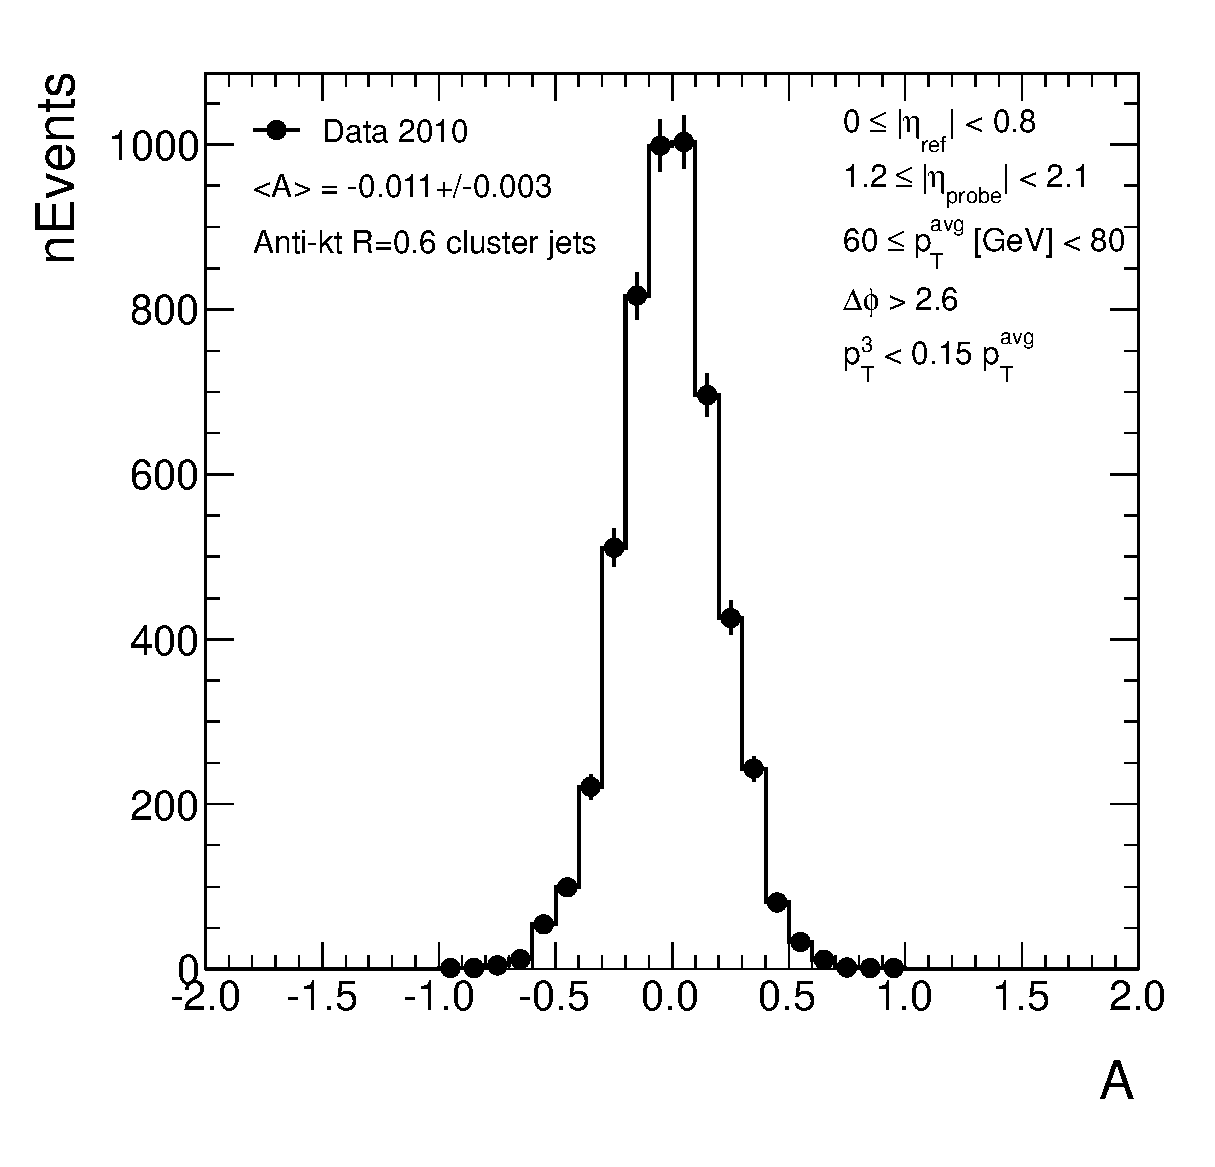
\includegraphics[width=\mediumfigwidth]{chapters/eta-intercalibration/Data.AntiKt6.refJetEta0_0.8.probeJetEta1.2_2.1.PTBinned.60_80.eps}
  \caption{A sample \Asymmetry distribution using \akt jets with $R=0.6$ and
           requiring that $\DeltaPhi(j_1,j_2) > 2.6$ and $60 \leq \pTavg < \unit{80}{\GeV}$
           with the reference jet falling into the region $\absEta < 0.8$ and the
           probe jet into the region $1.2 \leq \absEta < 2.1$.}
  \label{fig:etaint:sample_A_distribution}
\end{figure}

\subsection{Intercalibration using a Central Reference Region with a Soft-Radiation Correction}
As already discussed, a disadvantage with the method outlined above is that the
effects of soft radiation are hard to quantify and hence hard to correct for.
One solution to this is to apply a series of increasing cuts on the \pT of the
third hardest jet in the event and to extrapolate the information to the case in
which the third jet has zero \pT; in other words, the case in which there is no
soft radiation in the event. As can be seen from \FigureRef{fig:etaint:sample_extrapolation},
this can be done using a simple linear fit. The contents of each bin are, by definition,
highly correlated, since each bin is a superset of the previous one. Accordingly,
the best fit line was obtained by taking the covariance between the points into
account and minimising:

\begin{equation}
  \chi^2(\theta) = \sum_{i,j=1}^n \left(y_i - f(x_i, \theta)\right) V^{-1}_{ij} \left(y_j - f(x_j, \theta)\right)
\end{equation}

\noindent with respect to $\theta$. Here $f(x_i,\theta)$ is a simple linear function
in $x_i$, with $\theta$ representing the two free variables. The covariance matrix
$V$ is estimated using $V_{ij} = \frac{c_{ij}}{\sqrt{n_i n_j}}$, where $c_{ij}$ is the number
of events held in common between points $i$ and $j$ while $n_i$ and $n_j$ are the
total number of events contributing to each of these points.

\begin{figure}[htpb]
  \subfloat[\Asymmetry distribution for $\pT(j_3) / \pTavg < 0.19$]{
    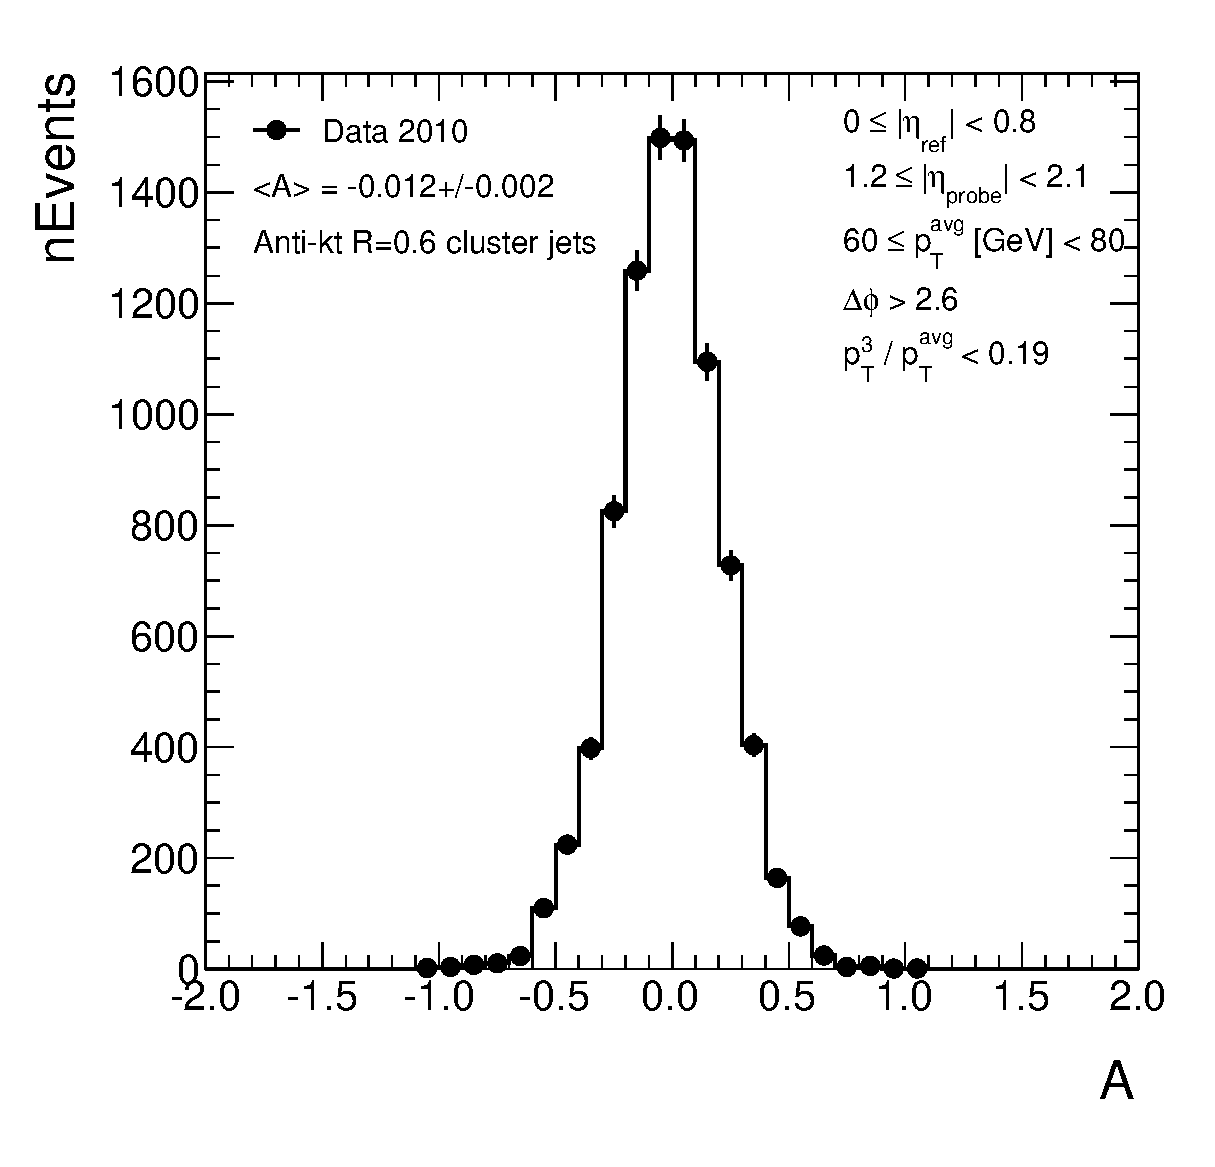
\includegraphics[width=\smallfigwidth]{chapters/eta-intercalibration/Data.AntiKt6.refJetEta0_0.8.probeJetEta1.2_2.1.PTBinned60_80.pT3_0.19.eps}
    \label{fig:etaint:sample_A_distribution_with_pT3_cut}}
  \quad
  \subfloat[Extrapolation to $\pT(j_3) = 0$]{
    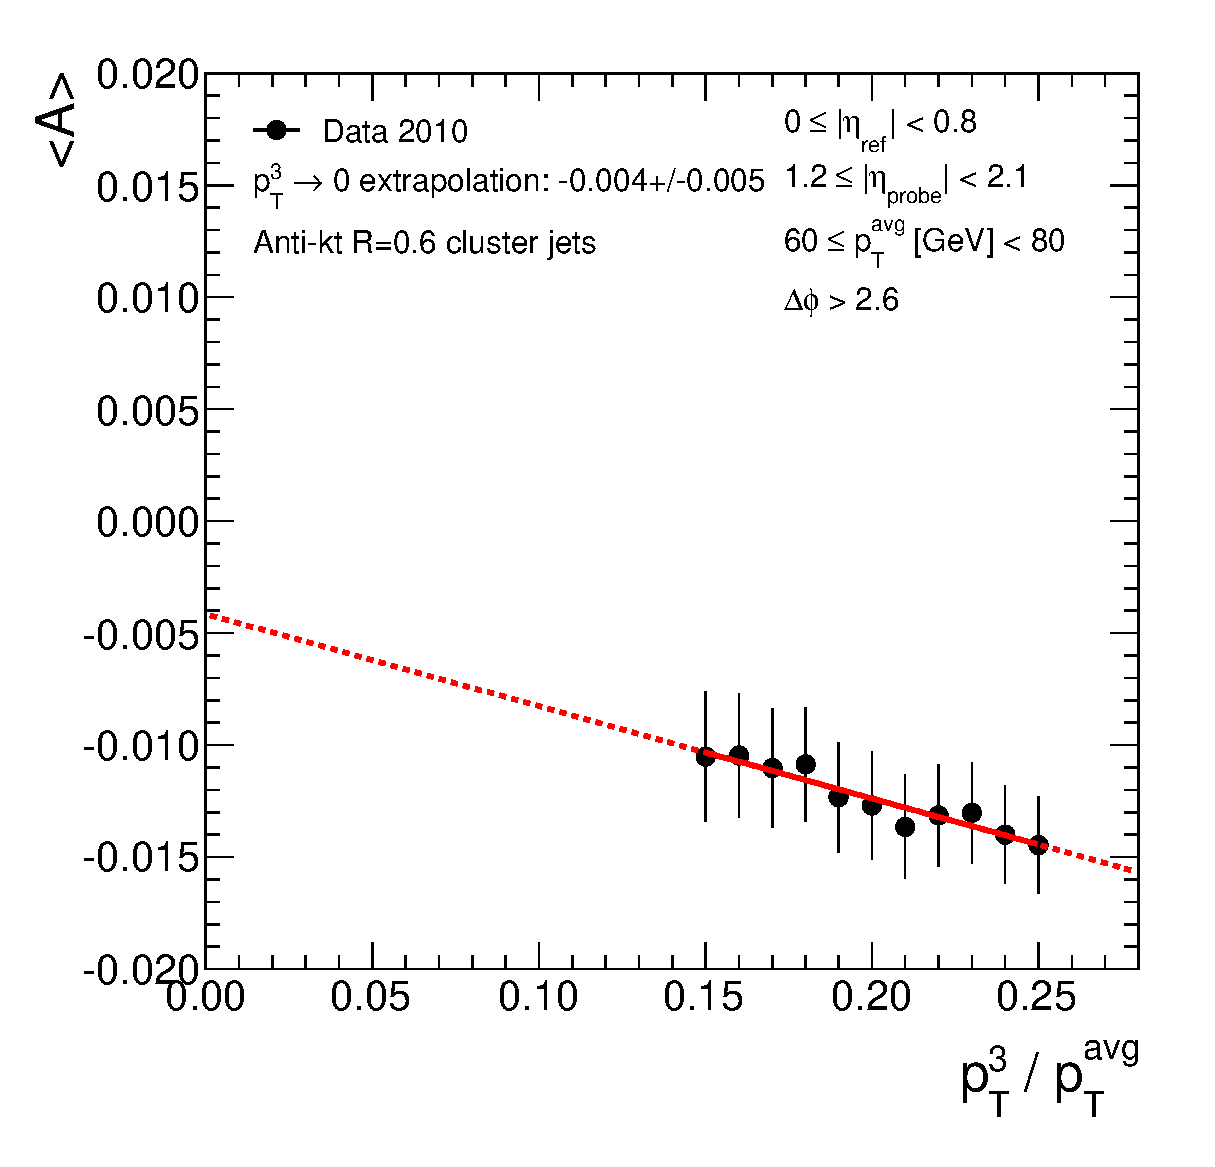
\includegraphics[width=\smallfigwidth]{chapters/eta-intercalibration/Data.AntiKt6.Extrapolation.refJetEta0_0.8.probeJetEta1.2_2.1.PTBinned.60_80.eps}
    \label{fig:etaint:sample_extrapolation}}
  \caption{A sample \Asymmetry distribution using \akt jets with $R=0.6$ and requiring
           that $\DeltaPhi(j_1,j_2) > 2.6$ and $60 \leq \pTavg < \unit{80}{\GeV}$,
           with the reference jet falling into the region $\absEta < 0.8$ and the
           probe jet into the region $1.2 \leq \absEta < 2.1$. \protect\subref{fig:etaint:sample_A_distribution_with_pT3_cut}
           is the \Asymmetry distribution for events which additionally satisfy
           $\pT(j_3) / \pTavg < 0.19$, while \protect\subref{fig:etaint:sample_extrapolation}
           shows the extrapolation from several different cuts on $\pT(j_3) / \pTavg$
           to the case in which $\pT(j_3) = 0$.}
  \label{fig:etaint:sample_thirdjet_curves}
\end{figure}

\section{Event Selection}
As discussed in \SectionRef{sec:analysis-tools:data_selection}, events are
required to belong to a good run and to have at least one good primary vertex.
For this analysis, the vertex requirement is tightened: only events with exactly
one good primary vertex are considered.

Events are required to possess at least two jets above the jet reconstruction
threshold of \unit{7}{\GeV}. The event is rejected if either of the two leading
jets are flagged as ``bad'' or ``ugly'' by the standard loose jet cleaning cuts,
discussed in \SectionRef{sec:analysis-tools:jet_cleaning}.

A trigger is assigned for each event, based on the run period and on \pTavg of
the \dijet pair. If this trigger is passed then the event is accepted. In later
periods, instead of a single trigger per event, two triggers are assigned, one
from the forward trigger system and one from the central trigger system. The
thresholds are chosen such that the trigger efficiency for each specific region
of \pTavg is greater than 99\% and is approximately flat as a function of the
pseudorapidity of the probe jet. To cover the low \pT region, $\pT < \unit{40}{\GeV}$,
as well as in early data taking when the trigger rates were low, triggers from
the minimum bias stream are used. These require at least one hit in the Minimum
Bias Trigger Scintillators (MBTS), which cover the region $2.08 \leq \absEta < 3.8$.
Forward triggers are not used before period E5, due to calibration problems.

\TableRef{tab:etaint:triggers} summarises the triggers used in the \etaint
measurement as a function of \pTavg and run period. As outlined in \SectionRef{sec:analysis-tools:jet_selection_evolution},
the lowest prescaled fully efficient jet trigger in each \pTavg bin changes over
time. All of these triggers are over 99\% efficient in the relevant regions.

\begin{table}
\begin{center}
  \begin{tabular}{ l l l @{\hspace{1.5cm}}l }
  \pTavg range $[\GeV]$ & Period A*   & Period B--D & Period E1--4 \\
  \midrule
  20--40                & L1\_MBTS\_1 & L1\_MBTS\_1 & L1\_MBTS\_1  \\
  40--50                & L1\_MBTS\_1 & L1\_J5      & L1\_J5       \\
  50--110               & L1\_J10     & L1\_J10     & L1\_J10      \\
  110--160              & L1\_J30     & L1\_J30     & L1\_J30      \\
  160+                  & L1\_J55     & L1\_J55     & L1\_J55      \\
  \midrule
  \pTavg range $[\GeV]$ & Period E5--F        & \multicolumn{2}{l}{Period G--H}                            \\
  \midrule
  20--40                & L1\_MBTS\_1         & \multicolumn{2}{l}{EF\_mbMbts\_1\_eff}                    \\
  40--50                & L1\_J5              & \multicolumn{2}{l}{EF\_mbMbts\_1\_eff}                    \\
  50--110               & L1\_J10 or L1\_FJ10 & \multicolumn{2}{l}{EF\_j30\_jetNoEF or EF\_fj30\_jetNoEF} \\
  110--160              & L1\_J30 or L1\_FJ30 & \multicolumn{2}{l}{EF\_j50\_jetNoEF or EF\_fj50\_jetNoEF} \\
  160+                  & L1\_J55 or L1\_FJ30 & \multicolumn{2}{l}{EF\_j75\_jetNoEF or EF\_fj75\_jetNoEF} \\
  \end{tabular}
  \caption{The trigger chains used for the \etaint analysis. The forward jet
           trigger could not be used in the first four periods (A--D) as it had
           not yet been commissioned, while additional problems made it
           unreliable for subperiods E1--4. L1\_MBTS\_1 was also used to trigger
           all jets before run 152777. The period after this timing change is
           denoted here as ``A*''.}
  \label{tab:etaint:triggers}
\end{center}
\end{table}

The \MC datasets which are compared to the data were generated using \Pythia,
\Herwigpp, \Alpgen and the \Perugia \Pythia tune, using the parameters described
in \SectionRef{sec:bg-theory:MC_generators}.

\section{\Dijet Balance Results}
In this section, the relative jet response obtained with the extrapolation
method is compared to the relative jet response obtained using the standard
method with a fixed cut on maximum $\pT(j_3)$. \FigureRef{fig:etaint:method_comparison_vs_eta}
shows the jet response relative to central jets, \relResponse, for two \pTavg-bins:
$30 \leq \pTavg < \unit{45}{\GeV}$ and $60 \leq \pTavg < \unit{80}{\GeV}$. These
results indicate that the response observed using the extrapolation method is
compatible with that obtained using the standard method. The results shown here
are representative of all the phase space regions considered in this analysis;
the extrapolation method is therefore used to give the final results for data
due to its more advanced treatment of residual soft effects; in the forward region,
where statistics in some \MC datasets are poor, this unfortunately results in large
errors.
%the standard method is retained for
%the \MC datasets as these suffer from poor statistics, particularly in the
%forward region.

\begin{figure}[htpb]
  \subfloat[$30 \leq \pTavg < \unit{45}{\GeV}$]{
    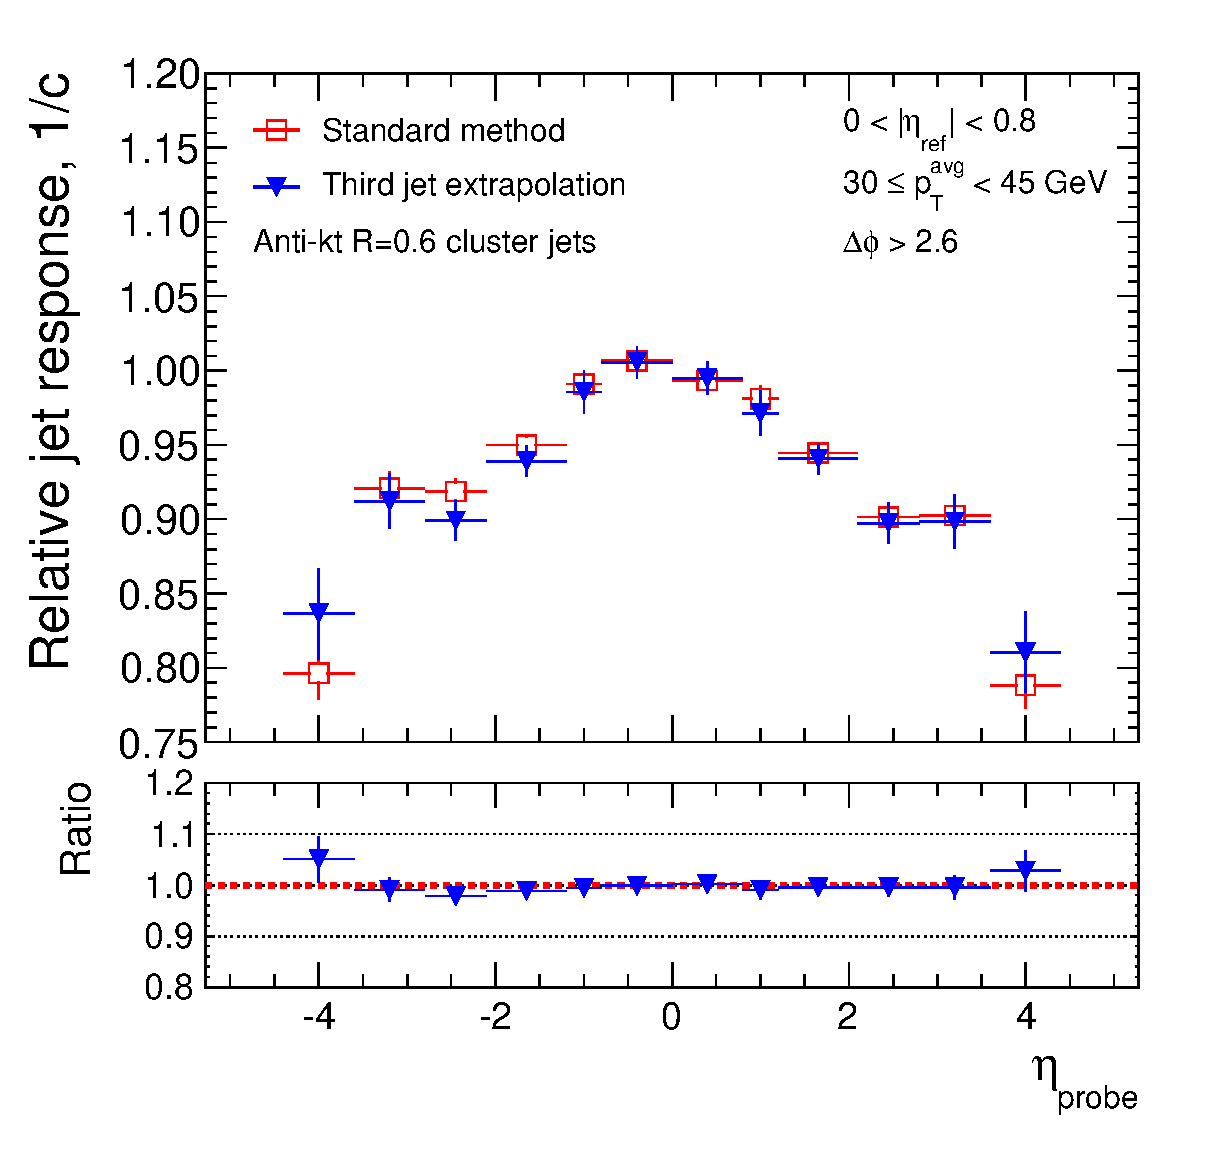
\includegraphics[width=\smallfigwidth]{chapters/eta-intercalibration/AntiKt6.refJetEta0_0.8.pTbar30_45.EtaBinned.MethodComparison.eps}
    \label{fig:etaint:method_comparison_vs_eta_pt30_45}}
  \quad
  \subfloat[$60 \leq \pTavg < \unit{80}{\GeV}$]{
    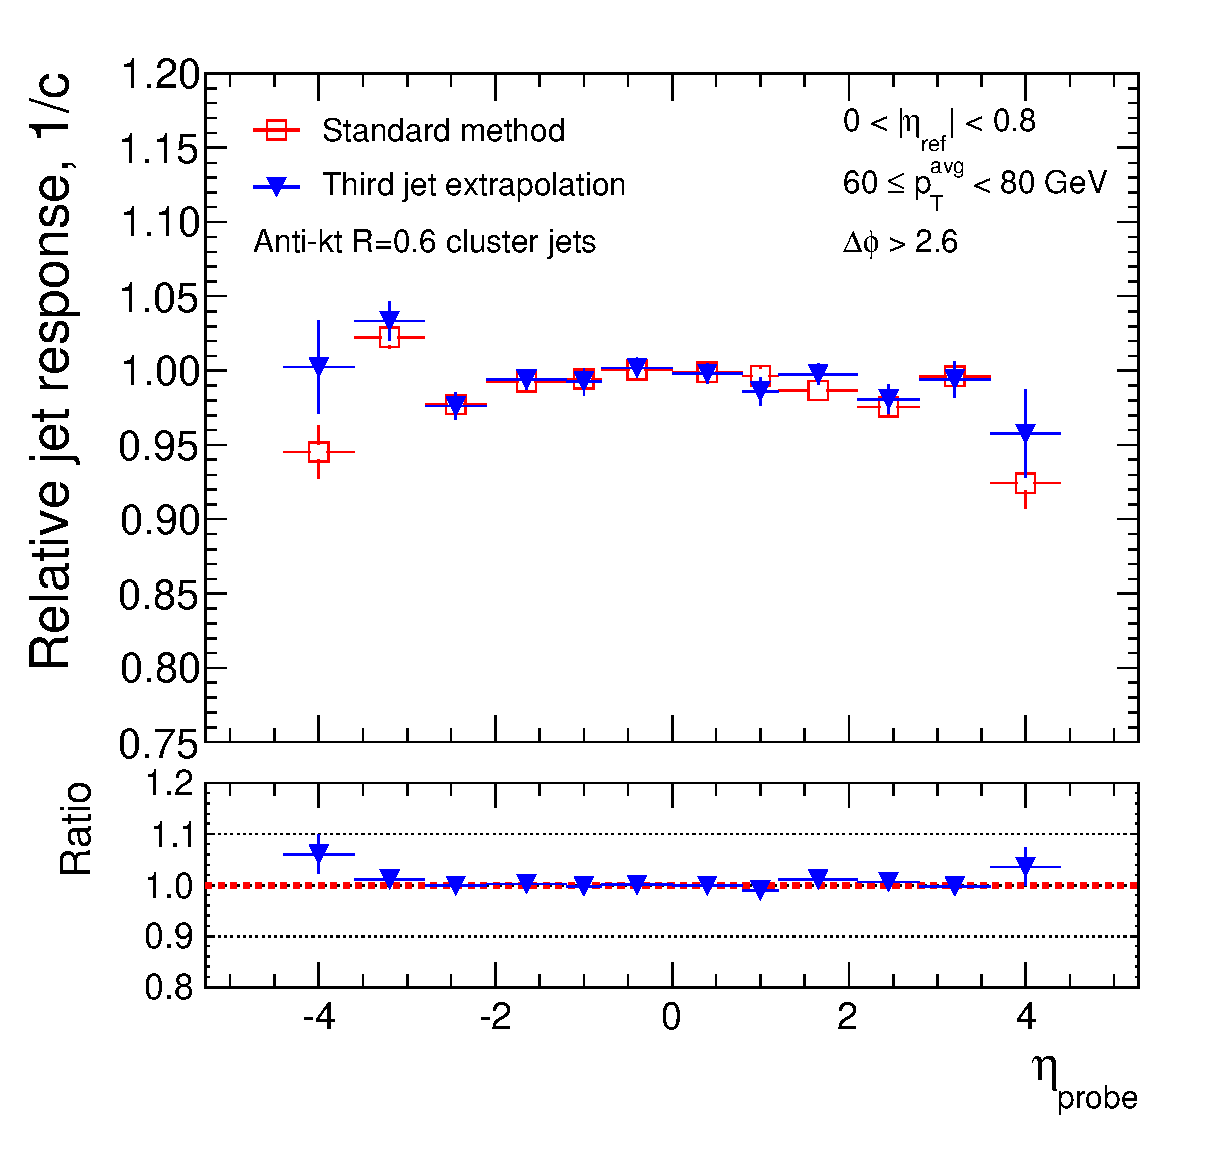
\includegraphics[width=\smallfigwidth]{chapters/eta-intercalibration/AntiKt6.refJetEta0_0.8.pTbar60_80.EtaBinned.MethodComparison.eps}
    \label{fig:etaint:method_comparison_vs_eta_pt60_80}}
  \caption{Relative jet response, 1/\relResponse, as a function of the
           pseudorapidity of the probe jet. Results are presented for two bins
           of \pTavg: \protect\subref{fig:etaint:method_comparison_vs_eta_pt30_45} $30 \leq \pTavg < \unit{45}{\GeV}$
           and \protect\subref{fig:etaint:method_comparison_vs_eta_pt60_80} $60 \leq
           \pTavg < \unit{80}{\GeV}$.}
  \label{fig:etaint:method_comparison_vs_eta}
\end{figure}

\FigureRef{fig:etaint:relative_jet_response_vs_eta} shows the relative response
obtained with the extrapolation method as a function of the jet pseudorapidity
for data and the \MC event generator simulations. Four different \pTavg regions
are shown: $20 \leq \pTavg < \unit{30}{\GeV}$, $30 \leq \pTavg < \unit{45}{\GeV}$,
$60 \leq \pTavg < \unit{80}{\GeV}$ and $80 \leq \pTavg < \unit{110}{\GeV}$. The
response in data is reasonably well reproduced by the \MC simulations for
$\pT > \unit{60}{\GeV}$, with the \MC and data typically agreeing at better than
the 2\% level in the central region ($\absEta < 2.8$) and better than 5\%
in the forward region ($\absEta > 2.8$). At lower values of \pTavg, the data
 do not agree so well with the \MC simulations and the \MC simulations
themselves show a large spread around the data. For $20 \leq \pT < \unit{30}{\GeV}$,
the \MC deviates from the data by about 10\% for $\absEta > 2.8$, with the
different \MC simulations predicting both higher and lower responses than that
observed in the data. The main differences, due to residual low \pT jet effects
(see \SectionRef{sec:etaint:central_reference}), occur between \Pythia/\Perugia
and \Alpgen/\Herwigpp. The reason is that the \Pythia and \Perugia predictions
are based upon a \pT-ordered parton shower, Lund String hadronisation and the
\Pythia underlying event model, whereas the \Herwigpp and \Alpgen predictions
are based on an angular-ordered parton shower, cluster hadronisation and the
\Jimmy underlying event model. These differences therefore reflect a 
difference in physics modelling among the event generators.

\begin{figure}[htpb]
  \subfloat[$20 \leq \pTavg < \unit{30}{\GeV}$]{
    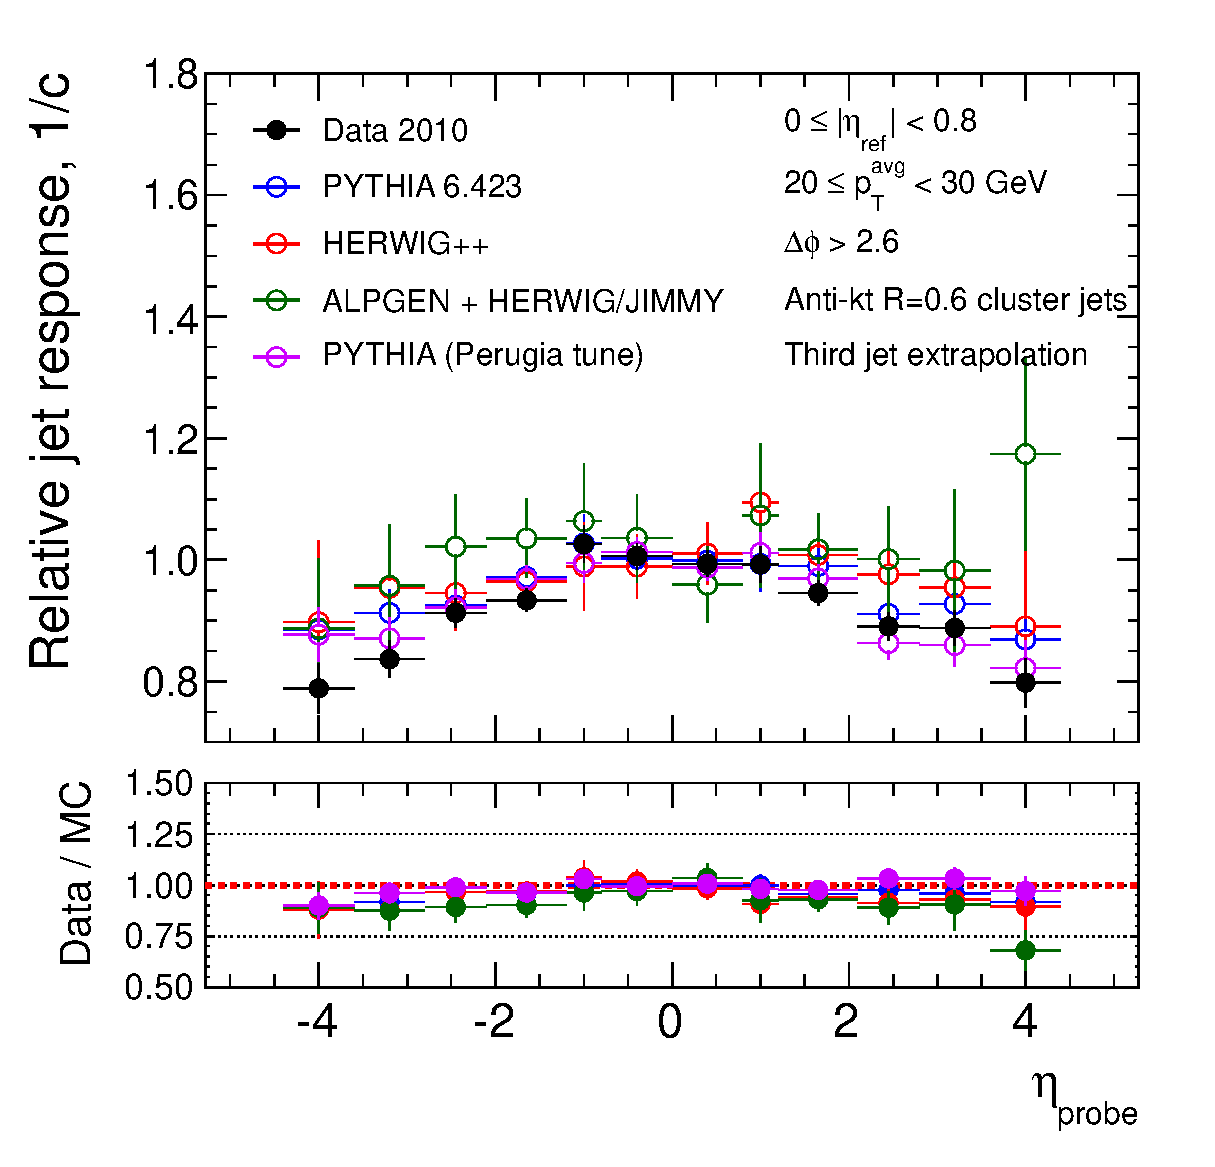
\includegraphics[width=\smallfigwidth]{chapters/eta-intercalibration/AntiKt6.refJetEta0_0.8.pTbar20_30.EtaBinned.ThirdJetExtrapolation.eps}
    \label{fig:etaint:relative_jet_response_vs_eta_pt20_30}}
  \quad
  \subfloat[$30 \leq \pTavg < \unit{45}{\GeV}$]{
    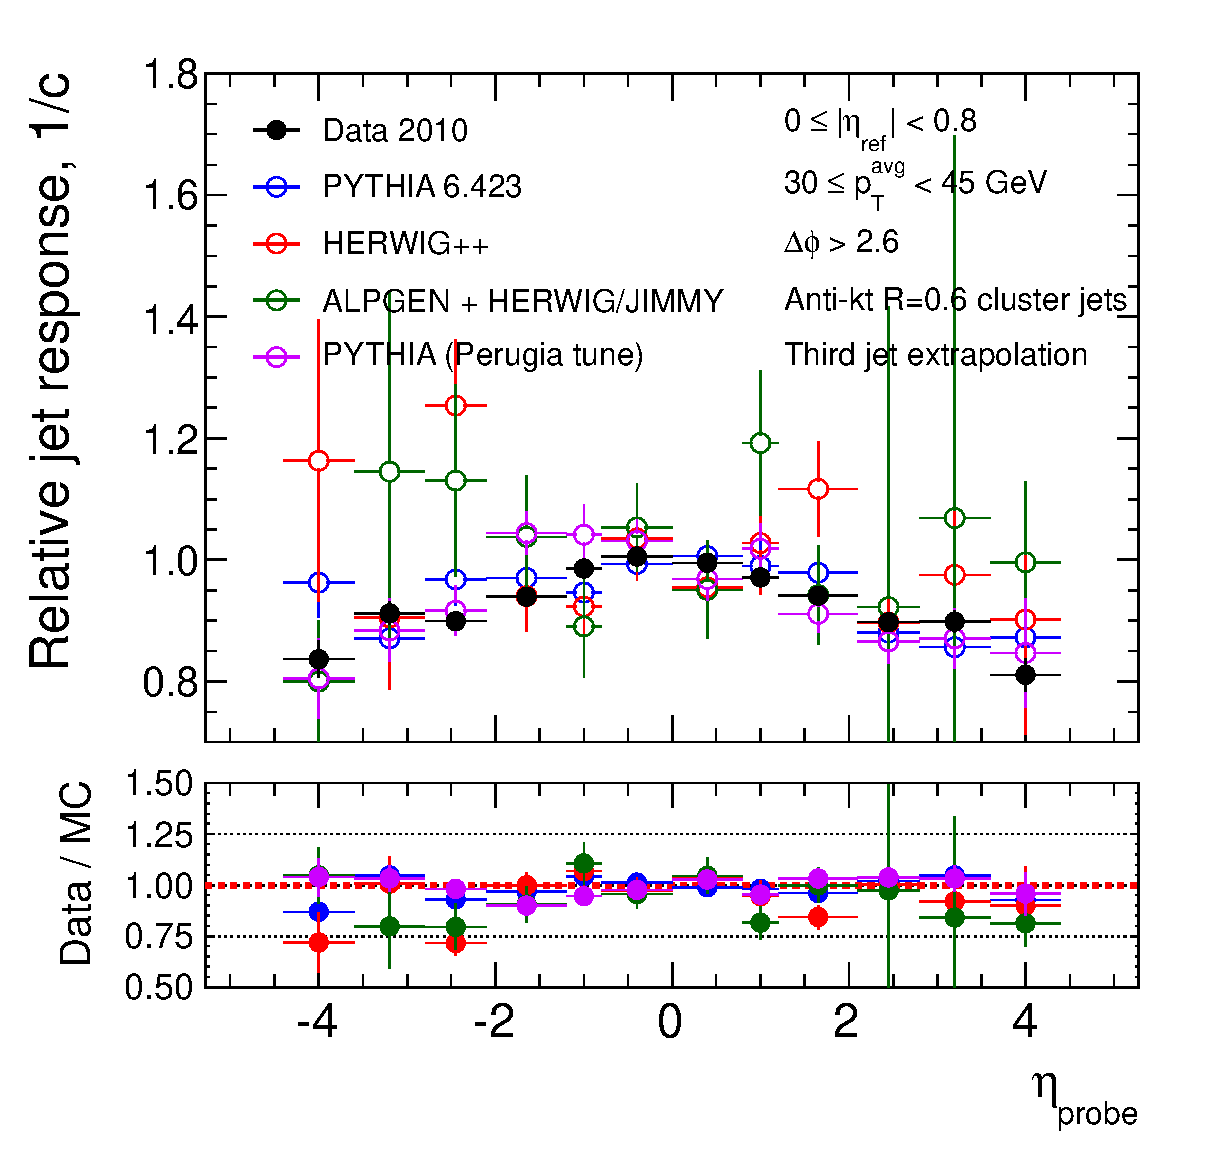
\includegraphics[width=\smallfigwidth]{chapters/eta-intercalibration/AntiKt6.refJetEta0_0.8.pTbar30_45.EtaBinned.ThirdJetExtrapolation.eps}
    \label{fig:etaint:relative_jet_response_vs_eta_pt30_45}}
  \\
  \subfloat[$60 \leq \pTavg < \unit{80}{\GeV}$]{
    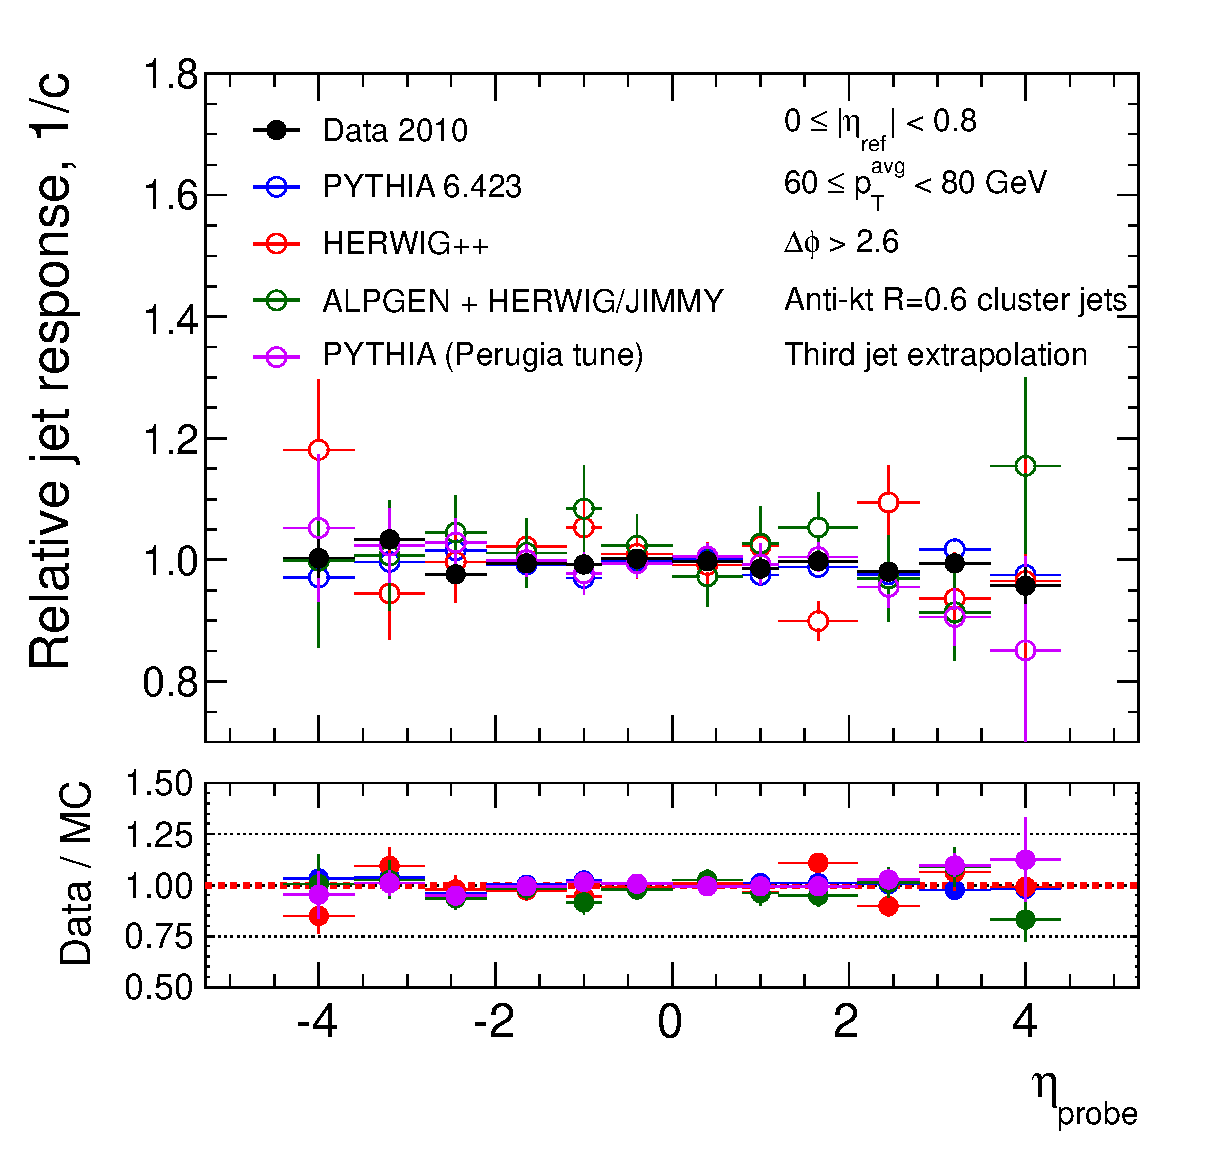
\includegraphics[width=\smallfigwidth]{chapters/eta-intercalibration/AntiKt6.refJetEta0_0.8.pTbar60_80.EtaBinned.ThirdJetExtrapolation.eps}
    \label{fig:etaint:relative_jet_response_vs_eta_pt60_80}}
  \quad
  \subfloat[$80 \leq \pTavg < \unit{110}{\GeV}$]{
    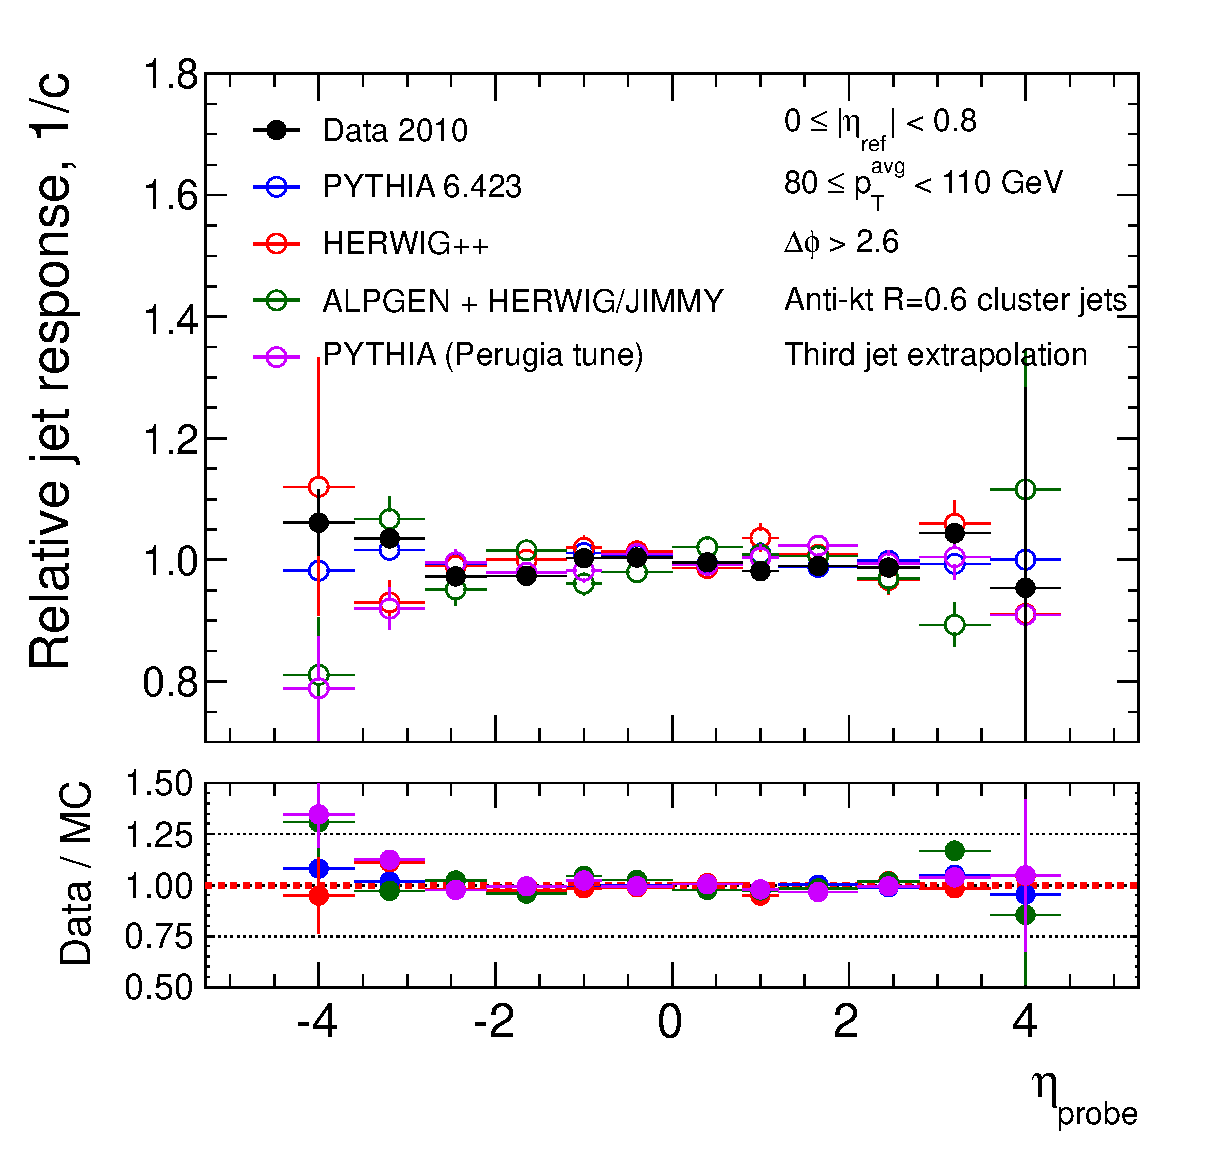
\includegraphics[width=\smallfigwidth]{chapters/eta-intercalibration/AntiKt6.refJetEta0_0.8.pTbar80_110.EtaBinned.ThirdJetExtrapolation.eps}
    \label{fig:etaint:relative_jet_response_vs_eta_pt80_110}}
  \caption{Relative jet response, 1/\relResponse, as a function of the \pseudorap
           of the probe jet. Results are presented for four bins of \pTavg:
           \protect\subref{fig:etaint:relative_jet_response_vs_eta_pt20_30} $20 \leq \pTavg < \unit{30}{\GeV}$,
           \protect\subref{fig:etaint:relative_jet_response_vs_eta_pt30_45} $30 \leq \pTavg < \unit{45}{\GeV}$,
           \protect\subref{fig:etaint:relative_jet_response_vs_eta_pt60_80} $60 \leq \pTavg < \unit{80}{\GeV}$
           and \protect\subref{fig:etaint:relative_jet_response_vs_eta_pt80_110} $80 \leq \pTavg < \unit{110}{\GeV}$.}
  \label{fig:etaint:relative_jet_response_vs_eta}
\end{figure}

\FigureRef{fig:etaint:relative_jet_response_vs_pt} shows the relative response as
a function of \pTavg. The distributions are shown for jets in the region $1.2 \leq \absEta < 2.1$
and also for those in the region $3.6 \leq \absEta < 4.4$. Again, the response
is reasonably well described by the \MC for all calorimeter regions at high
\pTavg and for the more central region at low \pTavg.

\begin{figure}[htpb]
  \subfloat[$1.2 \leq \absEta < 2.1$]{
    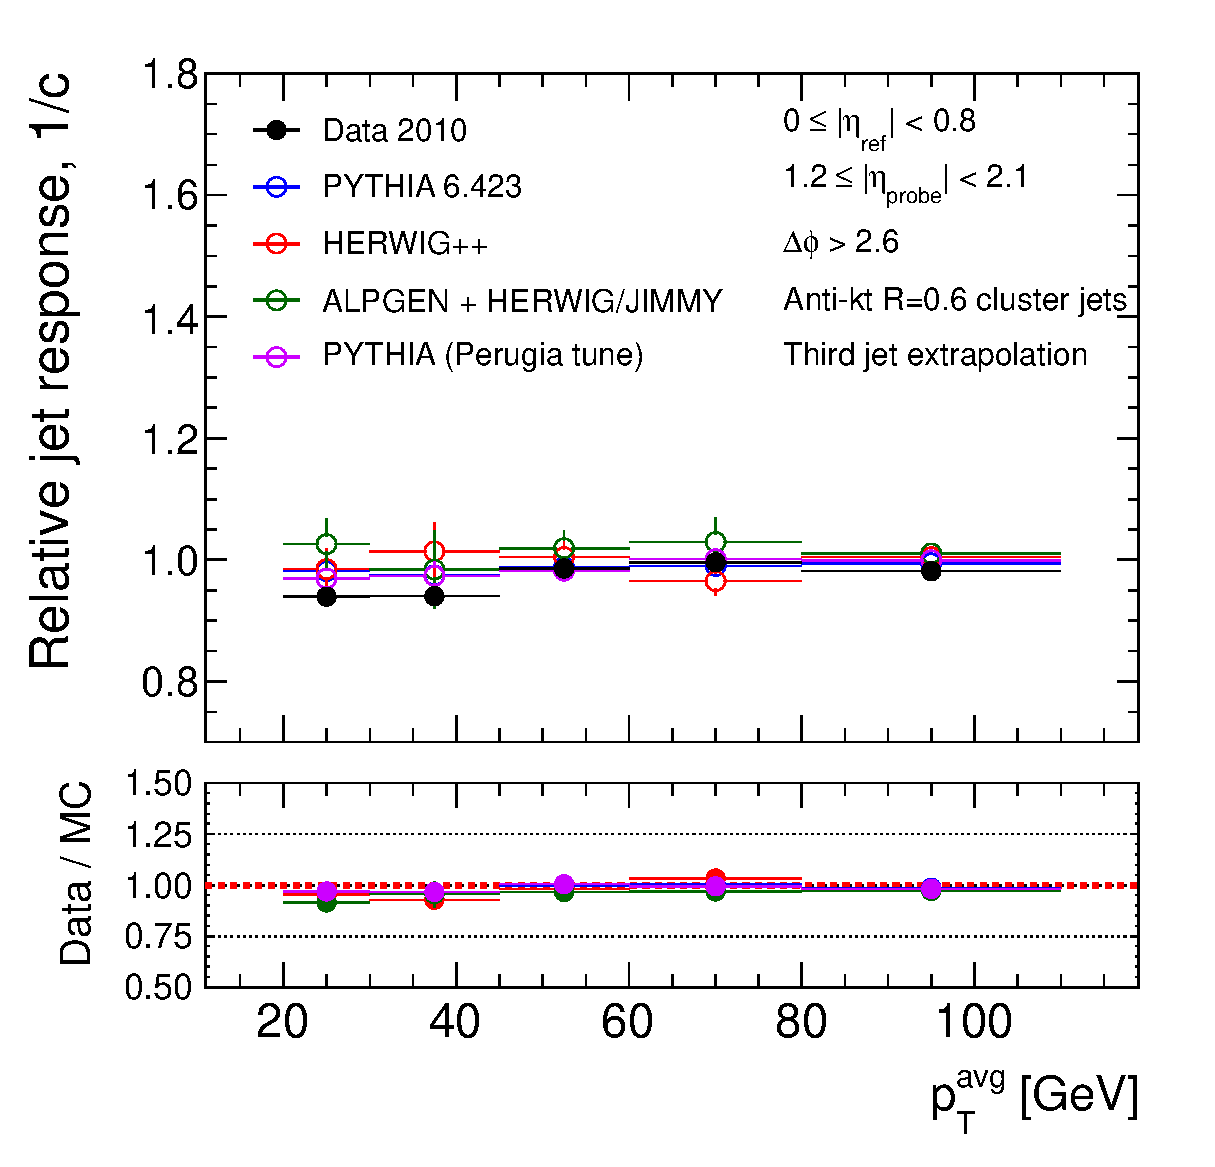
\includegraphics[width=\smallfigwidth]{chapters/eta-intercalibration/AntiKt6.refJetEta0_0.8.probeJetEta1.2_2.1.PTBinned.ThirdJetExtrapolation.eps}
    \label{fig:etaint:relative_jet_response_vs_pt_eta1.2_2.1}}
  \quad
  \subfloat[$3.6 \leq \absEta < 4.4$]{
    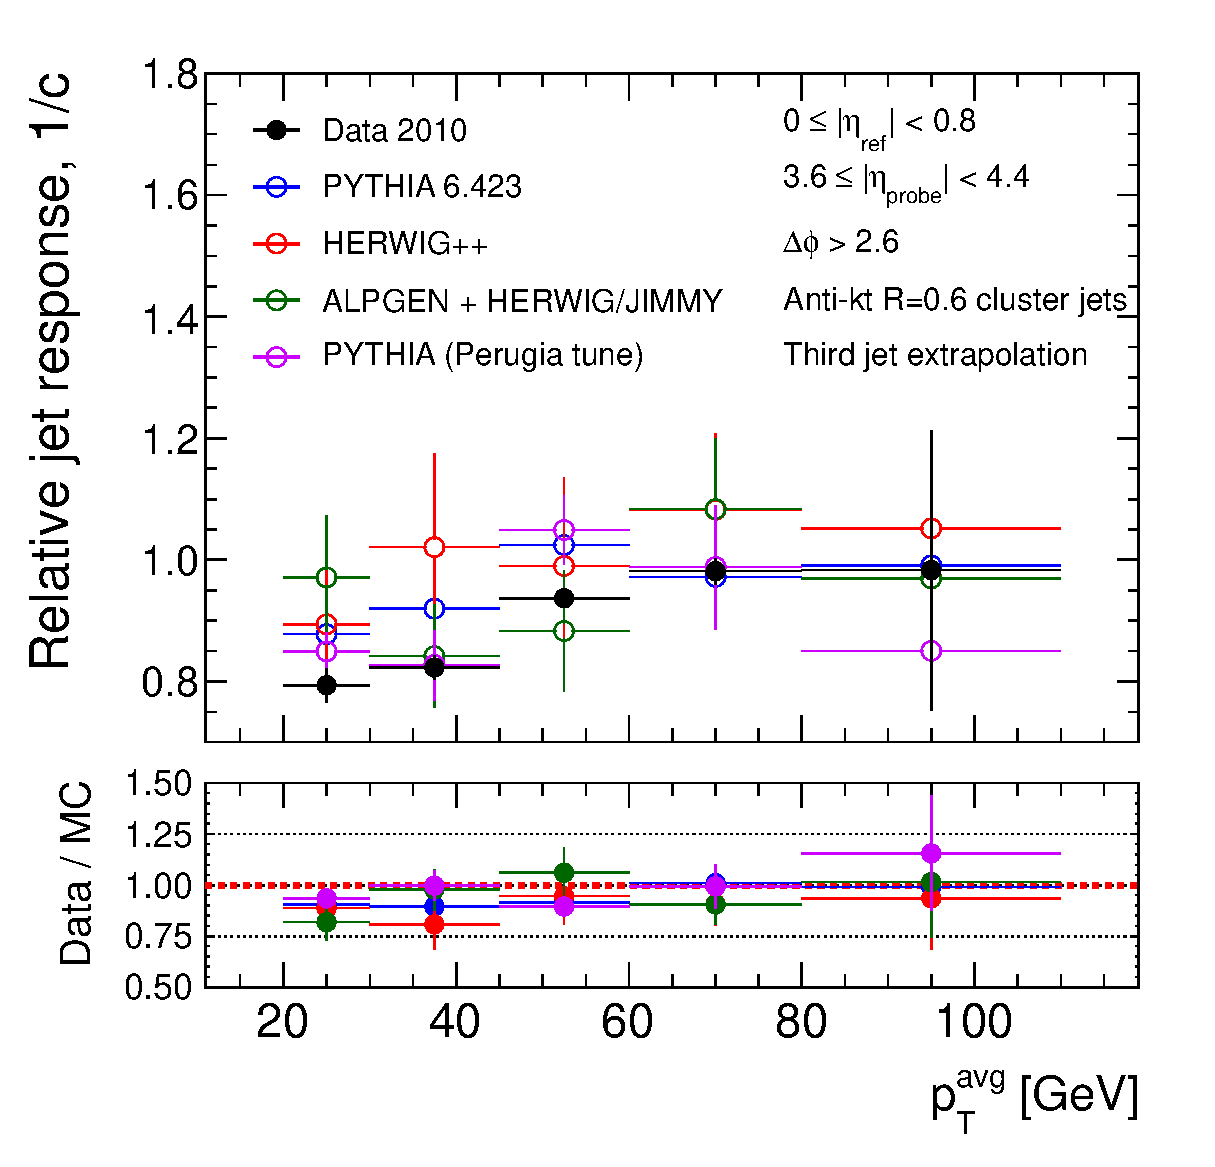
\includegraphics[width=\smallfigwidth]{chapters/eta-intercalibration/AntiKt6.refJetEta0_0.8.probeJetEta3.6_4.4.PTBinned.ThirdJetExtrapolation.eps}
    \label{fig:etaint:relative_jet_response_vs_pt_eta3.6_4.4}}
  \caption{Relative jet response, 1/\relResponse, as a function of the \pseudorap of the probe jet.
           For low \pTavg and early data periods, the data is collected using the minimum bias trigger stream. For
           higher \pTavg, the data is collected using the calorimeter trigger stream.
           Results are presented for two bins of \absEta: \protect\subref{fig:etaint:relative_jet_response_vs_pt_eta1.2_2.1}
           $1.2 \leq \absEta < 2.1$ and \protect\subref{fig:etaint:relative_jet_response_vs_pt_eta3.6_4.4}
           $3.6 \leq \absEta < 4.4$.}
  \label{fig:etaint:relative_jet_response_vs_pt}
\end{figure}


\section{Uncertainty due to Intercalibration}
In the previous section it was shown that the \MC predictions for the relative
jet response diverge at low values of \pTavg, with the data itself lying between
the different predictions for central values of \pseudorap. The uncertainty on
the relative jet response must reflect this disagreement because there is no \textit{a priori} reason to
believe one theoretical prediction over another. The uncertainty on the relative
response is taken to be the RMS deviation of the \MC predictions from the data.
At high \pTavg, where the spread of the \MC predictions is small, the
uncertainty mainly reflects the true difference between the response in data and
simulation. At low \pTavg and large \absEta, the uncertainty mainly reflects the
physics modelling uncertainty, although the detector-based differences between
data and simulation are also accounted for. The RMS spread of \MC predictions
around the data measurement is less sensitive to statistical fluctuations in
comparison to other possible measures of the deviation, such as the maximal
difference between the predictions or between data and \MC. The latter
quantities tend to give unstable results since all of the \MC samples used
in the analysis, aside from \Pythia, are generated with low statistics (for details see
\SectionRef{sec:bg-theory:MC_generators}); \MC generators with fewer than ten
entries in a particular bin of $|\etaProbe|$ and \pTavg are excluded from that bin
of the RMS calculation for this reason.

\begin{figure}[htpb]
  \subfloat[Uncertainty in the jet response as a function of \dijet \pTavg in five regions of the calorimeter.]{
    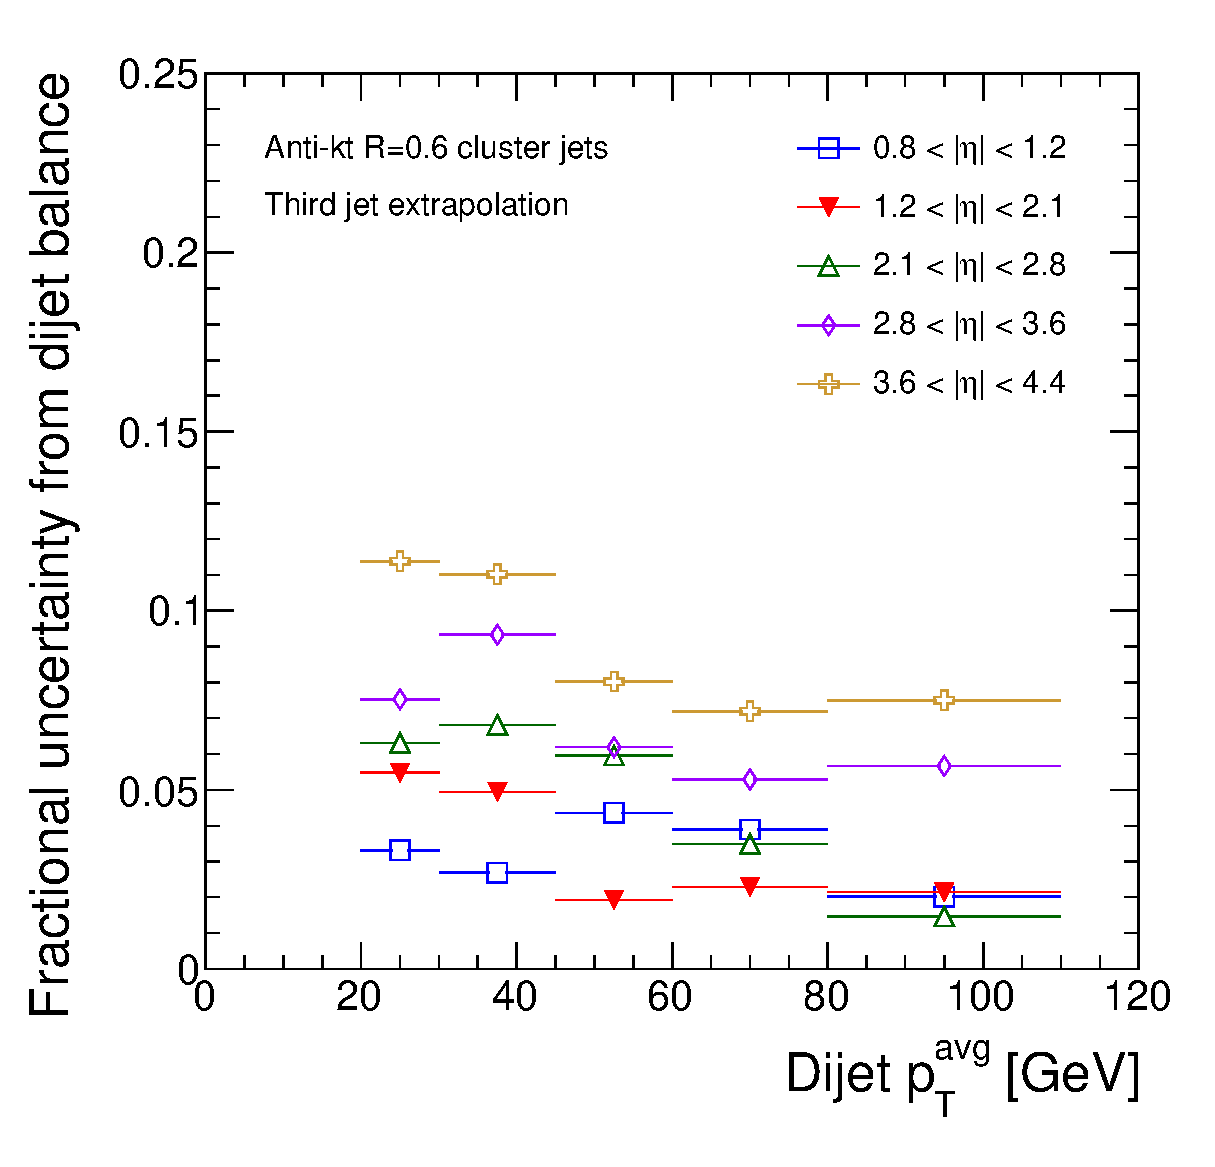
\includegraphics[width=\smallfigwidth]{chapters/eta-intercalibration/AntiKt6.JetResponseUncertainty.PTBinned.eps}
    \label{fig:etaint:relative_jet_response_uncertainty_vs_pt}}
  \quad
  \subfloat[Uncertainty in the jet response as a function of jet $\absEta$ for five values of \dijet \pTavg.]{
    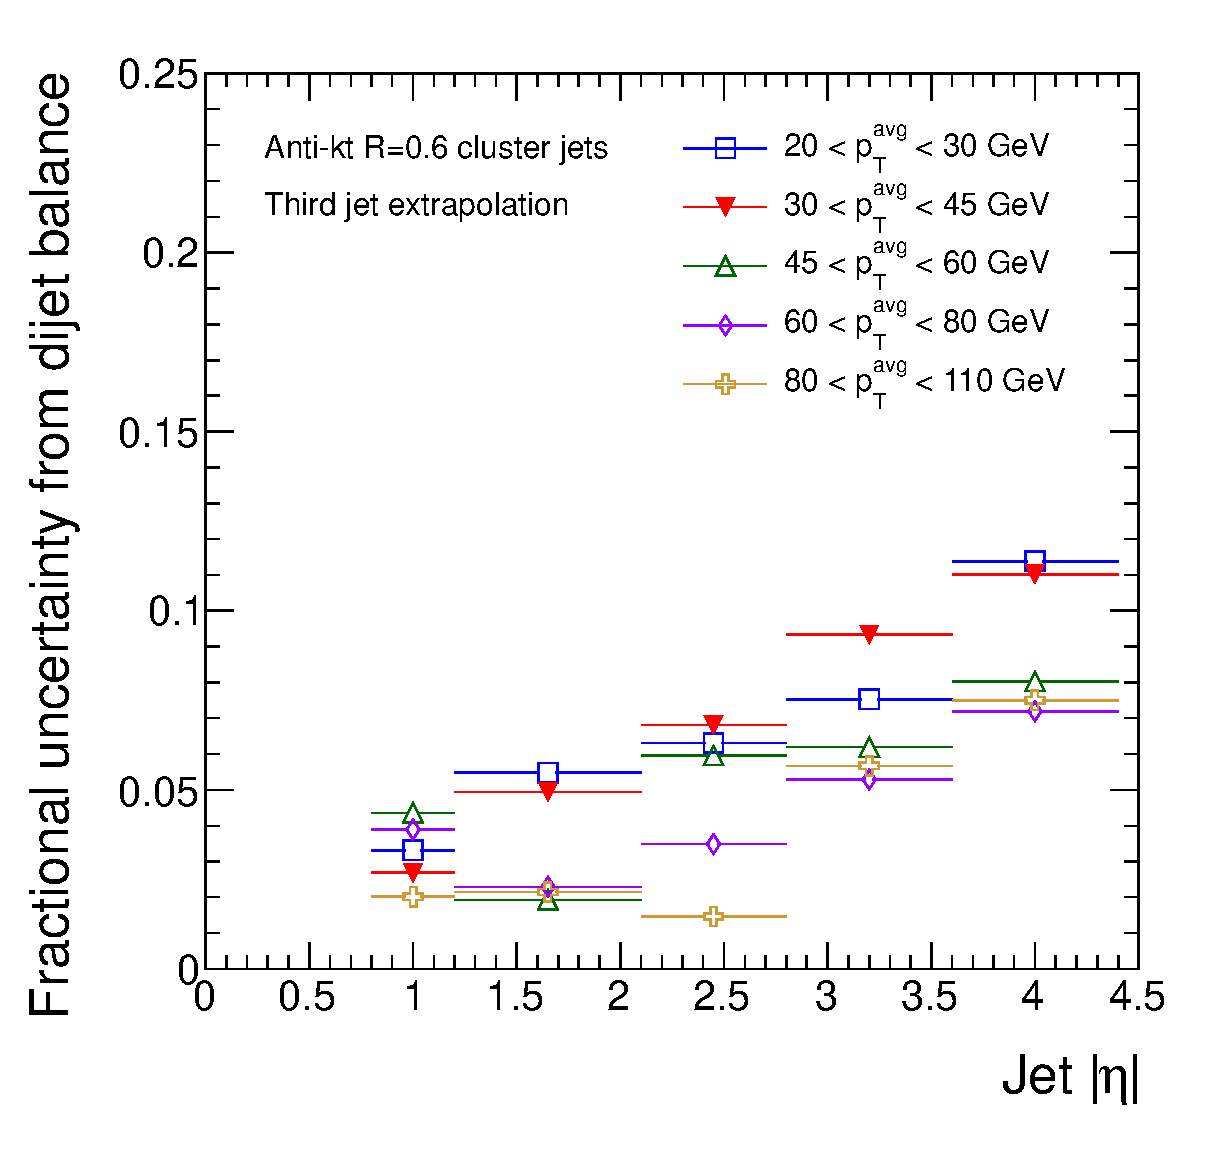
\includegraphics[width=\smallfigwidth]{chapters/eta-intercalibration/AntiKt6.JetResponseUncertainty.EtaBinned.eps}
    \label{fig:etaint:relative_jet_response_uncertainty_vs_eta}}
  \caption{Fractional uncertainty in the relative jet response, 1/\relResponse, arising from \dijet
           balance as a function of \protect\subref{fig:etaint:relative_jet_response_uncertainty_vs_pt} the \pTavg
           and \protect\subref{fig:etaint:relative_jet_response_uncertainty_vs_eta} the
           \pseudorap of the \dijet system.}
  \label{fig:etaint:relative_jet_response_uncertainty}
\end{figure}

\FigureRef{fig:etaint:relative_jet_response_uncertainty} shows the uncertainty in the jet response,
relative to jets in the region $\absEta < 0.8$, as a function of the \dijet \pTavg and $\absEta$.

\section{Summary}
These results indicate that the relative response to jets with $\absEta \leq 0.8$
is well understood both for high \pT jets across the full calorimeter range and
for central jets across the \pT range considered. Deviations between
data and \MC are at their smallest for high \pT central jets, at about 3\%, and
at their worst for low \pT forward jets, at about 12\%. Additionally, different
\MC generators show a large spread of predictions in the low \pT region,
reflecting a real physics modelling uncertainty. This work was published as an
\ATLAS conference note~\cite{ATLAS-CONF-2011-014} and also formed one of
the inputs for the evaluation of the jet energy scale 
uncertainty~\cite{ATLAS-CONF-2010-056} (see \SectionRef{sec:analysis-tools:jes_uncertainty} for details)
which was submitted to European Physical Journal C~\cite{CERN-PH-EP-2011-191}. The
results shown here are in agreement with these published results, which use a slightly
different method of determining the response factors, $1/c$, providing increased
statistical precision.
